%-----------------------------------------------------------------
\levelstay{Numbers}
\label{sec:Numbers}

% In this chapter, I'm listing a number of things I'm taken as \emph{given,} in
% the sense that I'm assuming we both know what I mean, without further
% explanation. 
% If you doubt the correctness of that assumption, I'll either provide a
% reference, or you can take the corresponding Wikipedia entry as good enough.
% 
% The main purpose for listing these things is to make it clear what I'm
% not going to explain, and, secondarily, to establish notation, though my intent
% is to stick to the most widely used notation, except when I given a reason not
% to.


%-----------------------------------------------------------------
\lstset{language=Clojure}

To establish notation:

The \textit{\gls{Integers}}: 
$\glssymbol{Integers} = \{\cdots, -2, -1, 0, 1, 2, \cdots\}$.

The \textit{\gls{NaturalNumbers}} (aka non-negative integers, aka counting
numbers):
$\glssymbol{NaturalNumbers} = \glsdesc{NaturalNumbers}$.\footnote{ 
Some
equate \gls{NaturalNumbers} with \glssymbol{PositiveIntegers} 
or $\glssymbol{NaturalNumbers}^{+}$ and use
$\glssymbol{NaturalNumbers}^{0}$ for the non-negative integers. 
See~\autoref{sec:math-sets} if the set specification
notation is new to you.}

The \textit{strictly positive integers}: 
$\glssymbol{PositiveIntegers} = \glsdesc{PositiveIntegers}$, which 
may also be written $\glssymbol{NaturalNumbers}^{+}$.

The \textit{\gls{RationalNumbers}}: 
$\glssymbol{RationalNumbers} = \glsdesc{RationalNumbers}$.

The \textit{\gls{RealNumbers}}, \glssymbol{RealNumbers},
can be defined in a number of ways. 
Qualitatively, \glssymbol{RealNumbers} is the completion of
\glssymbol{RationalNumbers}, in the sense it provides a limiting value for every
convergent sequence in \glssymbol{RationalNumbers}.

(Other number sets:
$\text{Constructible numbers} = \glssymbol{RationalNumbers}
+ \text{square roots}$

$\glssymbol{RationalNumbers}
\subset 
\text{Constructible Numbers}
\subset 
\glssymbol{RealNumbers}$.

Transcendental, Algebraic, \ldots.)

It should not be a surprise that:
$\glssymbol{NaturalNumbers} 
\subset 
\glssymbol{Integers}
\subset 
\glssymbol{RationalNumbers}
\subset 
\glssymbol{RealNumbers}$.
However, note that here we are silently assuming every integer
\emph{is} a real number, as opposed to considering \glssymbol{Integers} and
\glssymbol{RealNumbers} as distinct spaces, with the natural coercion
from \glssymbol{Integers} to a subset of \glssymbol{RealNumbers},
which is closer to how they are implemented.

Any of these ``number space'' symbols, \glssymbol{GenericSpace},
can be modified with sub-scripts to indicate restrictions or
extensions. 
(Using super-scripts here is more common --- I choose sub-scripts
to avoid confusion in things like $\aSpace{R}^{\infty}$,
which might be $\aSpace{R}$ extended with ${\infty}$, 
or might an infinite dimensional real vector space.)

For example, the spaces can be 
augmented by adding one or more values at infinity, which I will
write as $\glssymbol{GenericSpace}_{\infty}$,
or $\glssymbol{GenericSpace}_{\pm\infty}$ when I want to be 
clear that there are separate values for $-\infty$ and $+\infty$.

Or $\glssymbol{GenericSpace}_{+}$ ($\glssymbol{GenericSpace}_{-}$)
for the positive (negative) values, with 
$\glssymbol{GenericSpace}_{> 0}$, $\glssymbol{GenericSpace}_{\geq 0}$ 
when I feel the need to be clear about, eg, non-negative versus
strictly positive.

%-----------------------------------------------------------------
\leveldown{Generating spaces by 'closure'}

Generating these 'spaces' by closure under arithmetic operations
\cite{pickert-gorke-real-numbers-1974}.

A common pattern: a problem defined in terms of an existing mathematical
structure. Some combination of convenience, simplicity, computational
efficiency, and/or simplicity leads us to define a new structure, 
often a larger enclosing one.

We can use the number 'spaces' as an example.
Imagine, for the moment, that you only know the 
the natural numbers, $\glssymbol{NaturalNumbers}$, with a single operation: $+$.
Suppose we have a problem to solve:
\begin{math}
a + b = c
\end{math}
where $a,b,c\in \glssymbol{NaturalNumbers}$ and we know $b$ and $c$,
but not $a$.

%\begin{minipage}{\linewidth}
\begin{lstlisting}[
caption={[Re-inventing subtraction]Reinventing subtraction},
captionpos=b,
label=reinvent-subtraction,
mathescape=true,
%escapeinside={<*}{*>}
] 
(when (<= $b$ $c$)
  (loop [$a$ 0]
    (cond 
      (= $c$ (+ $a$ $b$)) $a$
      (< $c$ (+ $a$ $b$)) :no-solution
      :else (recur (+ 1 $a$)))))
\end{lstlisting}
%\end{minipage}

Rationals: 
\begin{math}
a * b = c
\end{math}

Reals: closure under sequence limit.
Suppose we have $x_0, x_1, \ldots \in \glssymbol{RealNumbers}$
where, for any $\epsilon>0$ there exists an $n$ such that
$|x_i - x_j| < \epsilon$ for any $i,, j > n$.

Insert example sequence that converges to $\sqrt{2}$ or $\pi$
with quick arg or ref to why it converges, but not to a rational
number.

%-----------------------------------------------------------------
\levelstay{Intervals}

Open and closed intervals, half open, etc.:
$[a,b] \subset \glssymbol{GenericSpace} = 
\setSpec{s \glssymbol{elementOf} \glssymbol{GenericSpace}}
{a \leq s \leq b}$;
$(a,b) \subset \glssymbol{GenericSpace} = 
\setSpec{s \glssymbol{elementOf} \glssymbol{GenericSpace}}
{a < s < b}$;
$[a,b) \subset \glssymbol{GenericSpace} = 
\setSpec{s \glssymbol{elementOf} \glssymbol{GenericSpace}}
{a \leq s < b}$;
and so on.

%-----------------------------------------------------------------
\levelstay{Java}
\lstset{language=Java}

%-----------------------------------------------------------------
\leveldown{Primitives}

%-----------------------------------------------------------------
\leveldown{Integers}
Finite subsets of \glssymbol{Integers} are exactly
represented by the primitive integer types using two's complement arithmetic, 
covering $[−2^{n−1}, 2^{n−1} − 1]$ where $n$ is the number of bits used:
\begin{description}
\item[\ttfamily {byte}] $8$ bits.
\item[\texttt{short}] $16$ bits.
\item[\texttt{int}] $32$ bits.
\item[\texttt{long}] $64$ bits.
\end{description}

Elements of \glssymbol{RealNumbers} are approximated using floating
point:
\begin{description}
\item[\texttt{float}] $32$ bits; range of finite values:
$\pm 3.40282347 x 10^{38}$, with special values for $\pm\infty$;
smallest non-zero value $1.40239846 x 10^{-45}$.
\item[\texttt{double}] $64$ bits;
range of finite values: 
$\pm 1.7976931348623157 x 10^{308}$, with special values for $\pm\infty$;
smallest non-zero value $4.9406564584124654 x 10^{-324}$.
\end{description}

%-----------------------------------------------------------------
\levelup{Objects}

\begin{figure}[htbp]
\centering
%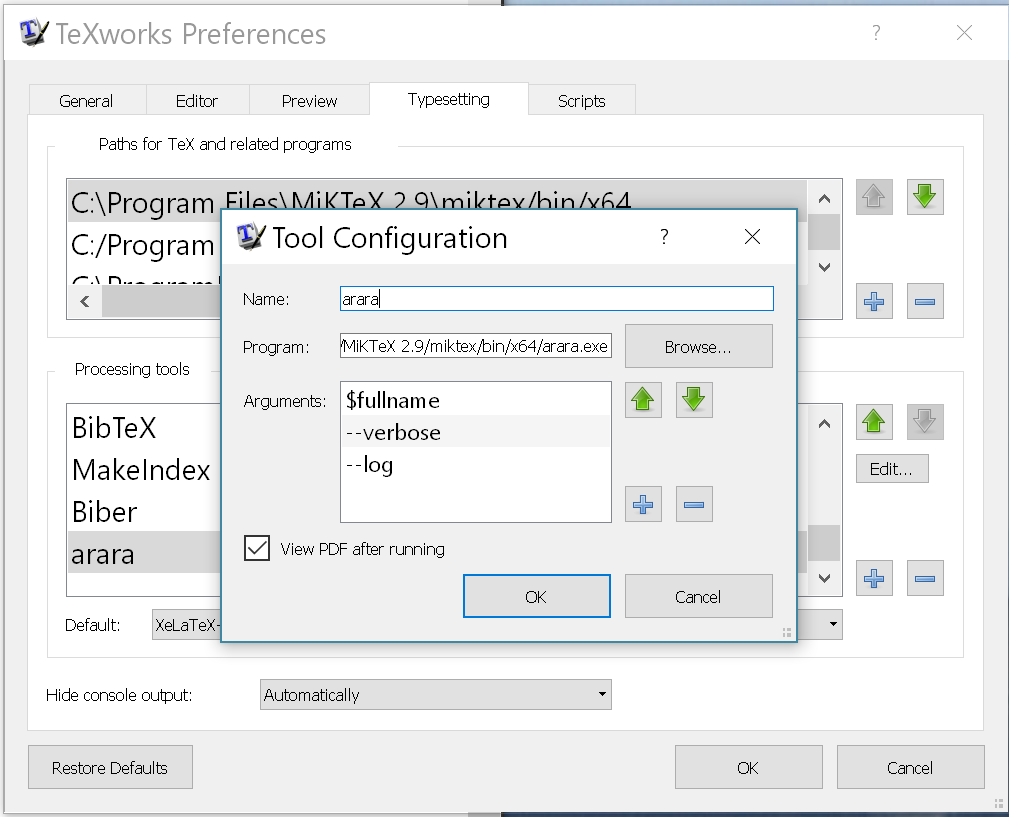
\includegraphics[scale=0.5]{figs/arara.png}
\caption{Java \texttt{Number} classes.}
\label{fig:java-number-classes}
\end{figure}

Boxed vs primitive arithmetic benchmark; 
int vs long vs float vs double vs Integer \ldots vs BigDecimal.


%-----------------------------------------------------------------
\levelup{Clojure}
\lstset{language=Clojure}

Clojure provides the primitive and boxed object numbers from Java,
except:
\begin{itemize}
  \item Full support for primitive type hints (eg for function arguments and
  return values) is only available for \lstinline|long| and \lstinline|double|.
  \item Idiomatic Clojure obscures whether primitive or boxed values will be
  used in any particular chunk of code (even more than recent versions  Java)
  Because of this, it is good practice to begin every namespace with
\begin{lstlisting}[
caption={[Boxed arithmetic warnings]}, label=unchecked-math,]  
(set! *unchecked-math* :warn-on-boxed)
\end{lstlisting}
which will generate compile-time warnings
\end{itemize}

Clojure adds rational numbers, which turn out to rarely be useful.\\
\lstinline|clojure.lang.Ratio| rational numbers
\lstinline|clojure.lang.BigInt|~\cite[p. 428]{Emerick2012ClojureProgramming}
